%------------------------------------
\chapter{Centrifugal Instability}
%------------------------------------
%------------------------------------
\section{The Oscillations of a Rotating Column of Liquid:}
%------------------------------------
Eliminating $u, v, w$ from the linearized perturbation equations (see \cite{drazin2004hydrodynamic} for details), we obtain the following equation and boundary conditions for the pressure perturbation  $\varpi$, where $p/\rho = \varpi e^{st + i(m\theta + k z)}$. In this problem $R_{1}=0$ and $R_{2}=R_{0}$. 

\begin{align}\label{eq:3_1_pressure_perturbation}
 \begin{split}
    \left(D_{*}D - \frac{m^{2}}{r^{2}} \right)\varpi &= k^{2}\left( 1 + \frac{4\Omega^{2}}{\gamma^{2}}\right)\\
    D\varpi + \frac{2im\Omega}{\gamma r} \varpi &= 0 \textrm{ at } r = R_{1}, r=R_{2} 
 \end{split}
\end{align}
where $D = d/dr, D_{*} = d/dr + 1/r$ and $\gamma = s + i m \Omega$. 

We rescale $r = \tilde{r}/R_{2}$ and let $a = kR_{2}$ to obtain
\begin{equation}\label{eq:3_1_bessel}
 \frac{d^{2}\varpi}{d\tilde{r}^{2}} + \frac{1}{\tilde{r}}\frac{d\varpi}{d\tilde{r}} + \left(-a^{2}\left( 1 + \frac{4\Omega^{2}}{\gamma^{2}}\right) - \frac{m^{2}}{\tilde{r}^{2}} \right)\varpi = 0
\end{equation}

This is the standard Bessel equation with solutions $\varpi(r) = A J_{m}(\alpha \tilde{r}) + B Y_{m}(\alpha \tilde{r})$. For regularity at $r=0$, we have $B = 0$. Here 
\begin{equation}\label{eq:3_1_alpha}
\boxed{\alpha^{2} = -a^{2}\left( 1 + \frac{4\Omega^{2}}{\gamma^{2}}\right)}. 
\end{equation}

Rescaling back to the original co-ordinates $r$, 
$\boxed{\varpi(r) = AJ_{m}(\alpha r/R_{2}) = AJ_{m}(\alpha r/R_{0})}$. 

The boundary condition applied at $r = R_{0}$ then implies that $\alpha$ must satisfy
\begin{equation}\label{eq:3_1_bc}
 \alpha J'_{m}(\alpha) + \frac{2im\Omega}{\gamma} J_{m}(\alpha) = 0.
\end{equation}

But from Eqn. (\ref{eq:3_1_alpha}), 
\begin{equation}\label{eq:3_1_alpha_inverted}
 \frac{2i\Omega}{\gamma} = \pm \sqrt{1 + \alpha^{2}/a^{2}} 
\end{equation}

Substituting Eqn.(\ref{eq:3_1_alpha_inverted}) into Eqn.(\ref{eq:3_1_bc}), $\alpha$ should be a root of the following equation:
\begin{equation}
 \alpha J'_{m}(\alpha) \pm m (1 +  \alpha^{2}/a^{2})^{1/2} J_{m}(\alpha) = 0
\end{equation}

Also, from Eqn.(\ref{eq:3_1_alpha_inverted}) and using the fact that $\gamma = s + im$, the frequencies of oscillations are given by

\begin{equation}\label{eq:3_1_freq_of_oscillations}
 \boxed{\frac{s}{\Omega_{0}} = \pm \frac{2i}{(1 +  \alpha^{2}/a^{2})^{1/2}} - im}.
\end{equation}

For the graphs of $is/\Omega_{0}$ Pulkit Dubey (PD) has a mathematica code, which will be uploaded soon. Also, $\S 68$ of \cite{chandrasekhar1961hydrodynamic} goes through the same analysis and plots the dispersion relation as in Fig. (\ref{fig:rotating_col_dispersion_chandra}), where $\alpha_{m, j}$ is the $j^{th}$ zero of $J_{m}(x)$.

 \begin{figure}[H]
    \centering
    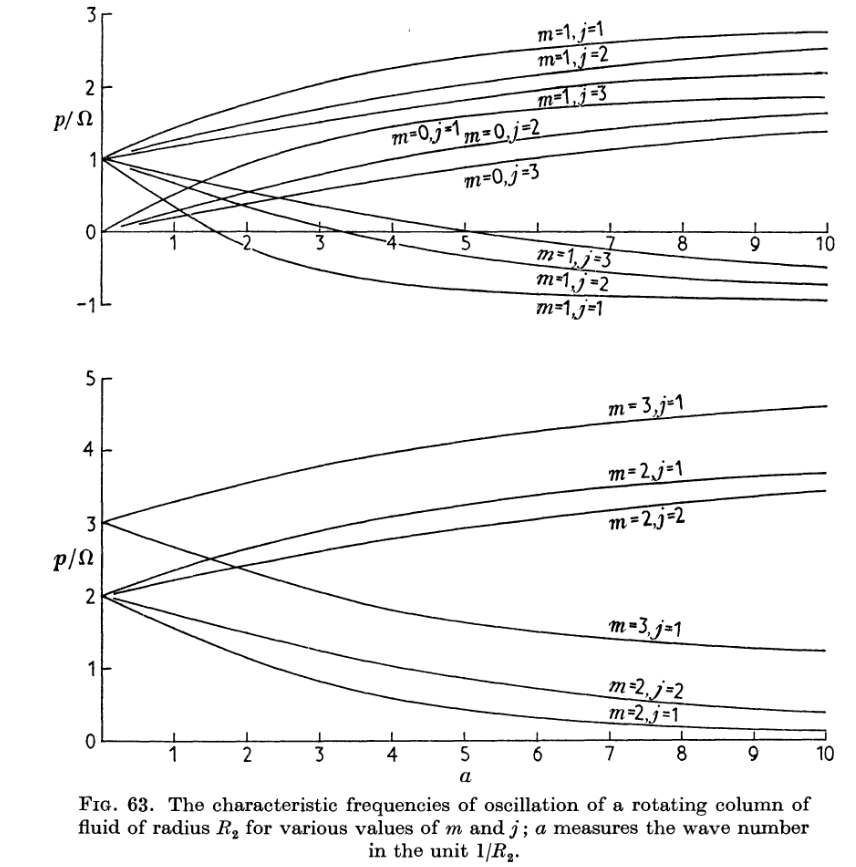
\includegraphics[scale = 0.4]{Figs/rotating_col_dispersion_chandra.png}
    \caption{Dispersion relation $is/\Omega_{0}$ vs. $a$, reproduced from \cite{chandrasekhar1961hydrodynamic}.}
    \label{fig:rotating_col_dispersion_chandra}
\end{figure}
